\documentclass[11pt,a4paper]{article}

\usepackage[margin=2cm,top=2.2cm,bottom=2.2cm]{geometry}
\usepackage{graphicx}
\usepackage{adjustbox}
\usepackage{titlesec}
\usepackage{enumitem}
\usepackage{hyperref}
\usepackage{fancyhdr}
\usepackage{xcolor}
\usepackage{setspace}
\usepackage{helvet}
\usepackage[T1]{fontenc}
\usepackage{tikz}
\usepackage{float}
\usepackage{placeins}
\usepackage{pdflscape}
\usepackage{caption}
\usepackage{booktabs}
\usepackage{longtable}
\usepackage{tabularx}
\usepackage{needspace}
\usepackage{array}
\usepackage{listings}

\setlength{\parskip}{0.45em plus 0.1em minus 0.05em}
\setlength{\parindent}{0pt}
\captionsetup{font=small, labelfont=bf, skip=6pt}
\floatplacement{figure}{htbp}

\renewcommand{\familydefault}{\sfdefault}

\definecolor{brandblue}{HTML}{0c3472}
\definecolor{brandlight}{HTML}{c8d7eb}
\definecolor{textgray}{HTML}{475569}

\hypersetup{
    colorlinks=true,
    linkcolor=brandblue,
    urlcolor=brandblue,
    pdftitle={Revenue Navigator Technical Architecture Plan},
    pdfauthor={Revenue Navigator Engineering}
}

\pagestyle{fancy}
\fancyhf{}
\fancyhead[L]{\small\textcolor{textgray}{Revenue Navigator --- Technical Architecture}}
\fancyhead[R]{\small\textcolor{textgray}{Engineering Specification}}
\fancyfoot[C]{\small\textcolor{textgray}{\thepage}}
\renewcommand{\headrulewidth}{0.4pt}
\renewcommand{\footrulewidth}{0pt}

\titleformat{\section}{\Large\bfseries\color{brandblue}}{}{0em}{}[\titlerule]
\titleformat{\subsection}{\large\bfseries\color{brandblue}}{}{0em}{}
\titlespacing*{\section}{0pt}{1em}{0.5em}
\titlespacing*{\subsection}{0pt}{0.8em}{0.35em}

\lstset{
    basicstyle=\ttfamily\small,
    breaklines=true,
    frame=single,
    backgroundcolor=\color{brandlight!30}
}

\newcommand{\techblock}[3]{%
    \vspace{0.25em}
    \noindent\textbf{#1}\\[0.15em]
    #2
    \vspace{0.2em}
    \noindent\textit{Implementation note:} #3
    \vspace{0.35em}
}

\newcolumntype{L}[1]{>{\raggedright\arraybackslash\ttfamily\small}p{#1}}
\newcolumntype{Y}{>{\raggedright\arraybackslash}X}

\newcommand{\docfig}[5]{%
    \begin{figure}[#1]
        \centering
        \adjustbox{max width=\textwidth, max height=#2, center}{%
            \includegraphics{#3}%
        }%
        \caption{#4}
        \label{#5}
    \end{figure}%
}

\newcommand{\docfigsafe}[5]{%
    \Needspace{10\baselineskip}%
    \docfig{#1}{#2}{#3}{#4}{#5}%
}

\newcommand{\docfiglandscape}[4]{%
    \clearpage
    \begin{landscape}
        \thispagestyle{fancy}
        \begin{figure}[H]
            \centering
            \adjustbox{max width=0.92\linewidth, max height=0.75\textheight, center}{%
                \includegraphics{#1}%
            }%
            \caption{#2}
            \label{#3}
        \end{figure}
    \end{landscape}%
}

\newcommand{\makecover}{%
    \thispagestyle{empty}
    \begin{center}
        \vspace*{1.5cm}
        {\color{brandblue}\rule{\textwidth}{2pt}}\\[0.8cm]
        {\fontsize{28}{34}\selectfont\bfseries\color{brandblue} Revenue Navigator}\\[0.3cm]
        {\large Technical Architecture Plan}\\[1.2cm]
        {\fontsize{22}{28}\selectfont\bfseries Production Backend}\\[0.2cm]
        {\fontsize{22}{28}\selectfont\bfseries Engineering Specification}\\[1.5cm]
        {\large FastAPI \textperiodcentered\ PostgreSQL \textperiodcentered\ Redis \textperiodcentered\ MongoDB}\\[0.3cm]
        {\large LangChain \textperiodcentered\ LiteLLM \textperiodcentered\ LangGraph \textperiodcentered\ Twilio}\\[2cm]
        
\begin{tikzpicture}
            \fill[brandlight, rounded corners=4pt] (0,0) rectangle (10,1.2);
            \node at (5,0.6) {\textbf{\color{brandblue} Confidential --- Engineering Review}};
        \end{tikzpicture}\\[2cm]
        {\large \today}\\[0.5cm]
        {\color{textgray} Greenfield backend design derived from frontend product flows}
        \vfill
        {\color{brandblue}\rule{\textwidth}{2pt}}
    \end{center}
    \newpage
}

\begin{document}

\makecover

\tableofcontents
\newpage

% =============================================================================
\section{Executive Technical Summary}

\textbf{Revenue Navigator} requires a production-grade backend that unifies account intelligence, predictive scoring, lifecycle classification, and multi-channel outreach. This document specifies a \textbf{greenfield architecture}---independent of any prior prototype implementation---aligned with the React frontend in \texttt{revenue-navigator/}.

\subsection{Technology Stack}

\begin{itemize}[leftmargin=1.5em, itemsep=0.25em]
    \item \textbf{API:} FastAPI + Uvicorn (async HTTP, WebSocket voicebot)
    \item \textbf{Relational store:} PostgreSQL 15+ with Alembic migrations
    \item \textbf{Document store:} MongoDB (transcripts, raw payloads, LLM traces)
    \item \textbf{Cache \& queue:} Redis (cache, Celery broker, distributed locks, rate limits)
    \item \textbf{AI:} LangChain tools, LiteLLM model router, LangGraph state machines
    \item \textbf{Communications:} Twilio (voice, SMS, WhatsApp), transactional email provider
    \item \textbf{Jobs:} Celery Beat (cron), Celery workers (prefork/gevent pools)
\end{itemize}

\subsection{Non-Functional Requirements}

\begin{tabular}{@{}ll@{}}
\toprule
\textbf{Requirement} & \textbf{Target} \\
\midrule
API p95 latency (read) & $<$ 200\,ms \\
API p95 latency (dashboard aggregate) & $<$ 500\,ms (Redis-cached) \\
Scoring batch (10k accounts) & $<$ 30\,min \\
Webhook acknowledgment & $<$ 500\,ms (async processing) \\
Uptime & 99.5\% (single-region MVP) \\
Tenancy & Row-level \texttt{tenant\_id} on all core tables \\
\bottomrule
\end{tabular}

% =============================================================================
\section{System Context}

The frontend exposes these protected modules (from \texttt{App.tsx}):

\begin{itemize}[leftmargin=1.5em, itemsep=0.2em]
    \item \textbf{Dashboard} --- portfolio KPIs, lifecycle stage alerts, NBA queue
    \item \textbf{Accounts / Account Detail} --- CRUD, timeline, comments, ticket stats
    \item \textbf{Pipeline} --- Q1--Q4 renewal stages per vendor (zscaler, adobe, crowdstrike)
    \item \textbf{Sentiment} --- communication sentiment trends
    \item \textbf{Opportunities} --- upsell pipeline
    \item \textbf{Analytics} --- MRR, risk distribution, retention trends
    \item \textbf{Manual Triggers} --- on-demand ML, email, voice runs
    \item \textbf{Settings / Setup} --- schedule windows, credentials, lifecycle bucket config
\end{itemize}

Each module maps to backend bounded contexts documented in Section~4. The frontend calls \texttt{/api/v1/*}; WebSocket endpoints serve the browser voicebot.

% =============================================================================
\section{Platform Architecture}

Six logical layers isolate concerns and enable independent scaling (Figure~\ref{fig:platform}).

\begin{enumerate}[leftmargin=1.5em, itemsep=0.3em]
    \item \textbf{Presentation} --- React SPA; JWT in Authorization header
    \item \textbf{API Gateway} --- FastAPI routers, auth middleware, Redis rate limits, webhook signature validation
    \item \textbf{Domain Services} --- business logic packages; no direct LLM calls from route handlers
    \item \textbf{AI Orchestration} --- LangGraph graphs; LiteLLM routes to Azure OpenAI / OpenAI / Anthropic
    \item \textbf{Async Execution} --- Celery + Redis; APScheduler only for lightweight polls inside API process
    \item \textbf{Data} --- PostgreSQL (source of truth), MongoDB (unstructured), Redis (ephemeral)
\end{enumerate}

\begin{landscape}
\thispagestyle{fancy}
\begin{figure}[p]
    \vspace*{-0.8cm}
    \centering
    \adjustbox{max width=\linewidth, max height=0.76\paperheight, center}{%
        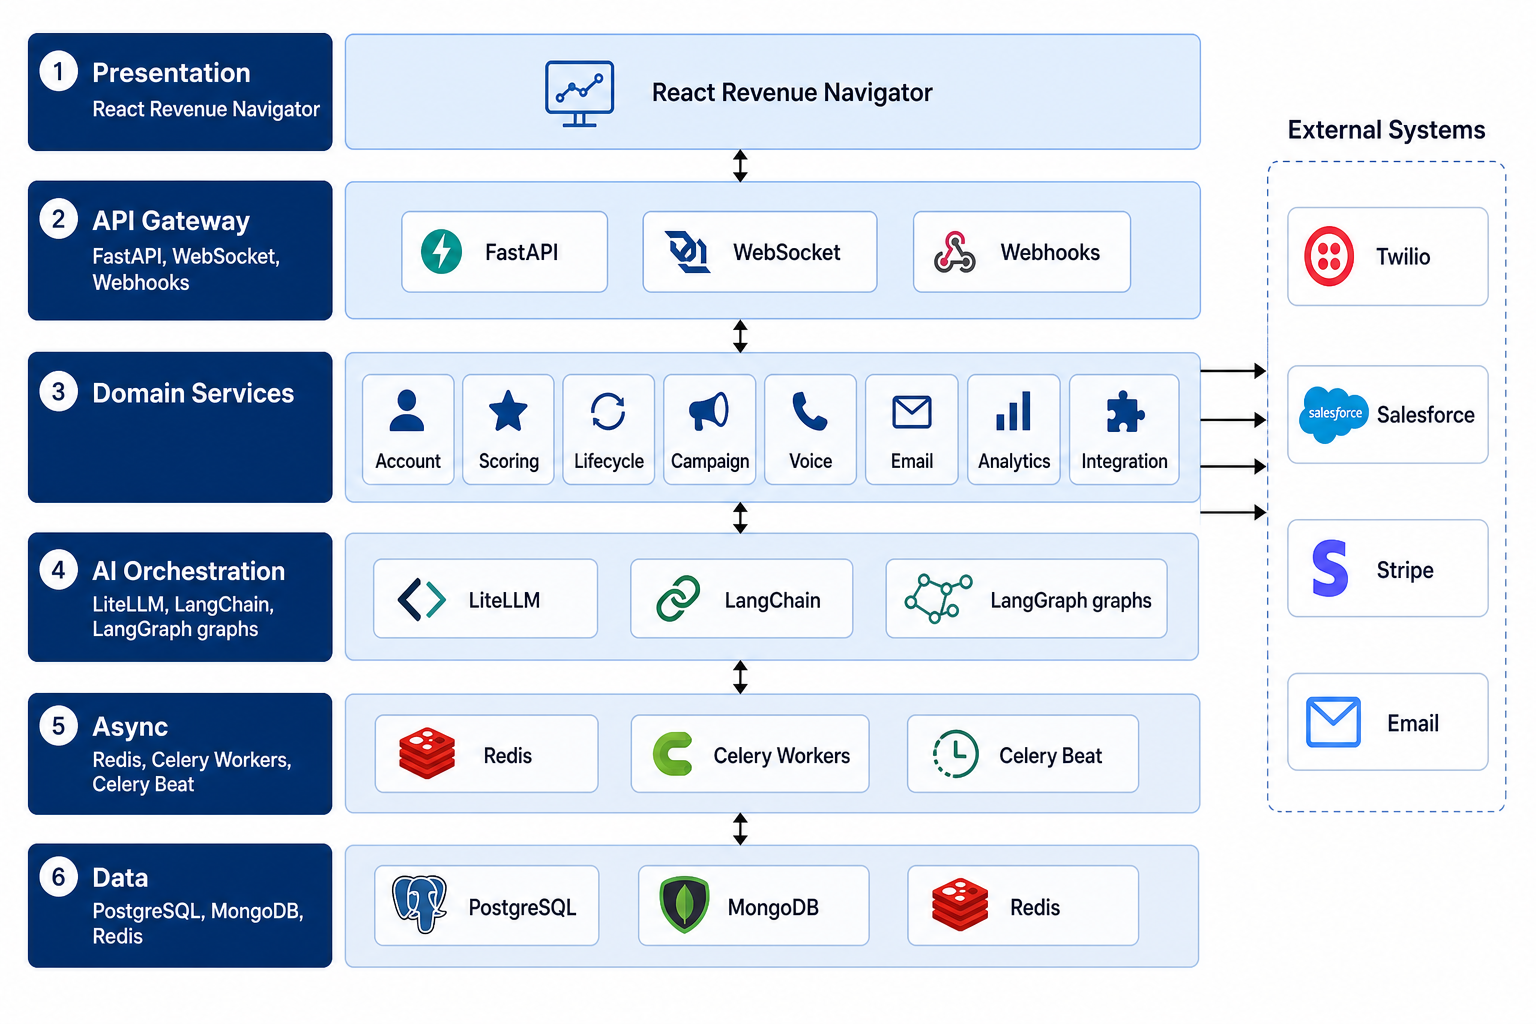
\includegraphics{images/rnu-tech-platform-architecture.png}%
    }
    \caption{Six-layer platform architecture --- presentation through data foundation with external integrations.}
    \label{fig:platform}
    \vspace*{-0.4cm}
\end{figure}
\end{landscape}

\FloatBarrier

\docfig{htbp}{0.42\textheight}{images/rnu-tech-data-flow.png}{End-to-end technical data flow --- ingest, score, act, feedback with store annotations.}{fig:dataflow}

% =============================================================================
\section{Service Decomposition}

Monolith-first: one FastAPI repository with \texttt{app/services/<domain>/} packages. Extract microservices when a worker pool requires independent scaling (voice workers first).

\begin{longtable}{@{}p{3.2cm}p{5.5cm}p{3.5cm}@{}}
\toprule
\textbf{Service} & \textbf{Responsibility} & \textbf{Primary Store} \\
\midrule
\endhead
account-service & CRUD, timeline, comments, ticket stats & PostgreSQL \\
scoring-service & Health, churn, relationship, renewal, upsell pipeline & PostgreSQL + ml\_score\_history \\
classification-service & Fit-ratio lifecycle bucket assignment (Protect--Activate) & PostgreSQL + Redis cache \\
lifecycle-service & NBA recommendations, pipeline grid aggregation & PostgreSQL + Redis cache \\
campaign-service & Auto-campaigns, filters, IST send windows & PostgreSQL \\
email-service & Outbound, inbound, intent, drip sequences & PostgreSQL + Mongo \\
voice-service & Twilio IVR, outbound calls, transcripts & PostgreSQL + Mongo \\
whatsapp-service & Twilio WhatsApp threads & PostgreSQL + Mongo \\
analytics-service & Portfolio aggregates, trends, CSV export & PostgreSQL (materialized views) \\
integration-service & Salesforce/Stripe sync, webhook normalization & PostgreSQL + Mongo \\
settings-service & App config, encrypted credential references & PostgreSQL \\
workflow-service & Q1--Q4 dynamic pipelines, step execution, Resend/Twilio dispatch & PostgreSQL \\
\bottomrule
\end{longtable}

\textbf{Package layout (target):}
\begin{lstlisting}
backend/
  alembic/
  app/
    api/v1/endpoints/
    core/          # config, security, logging
    db/            # SQLAlchemy session, base
    models/        # ORM (PostgreSQL only)
    schemas/       # Pydantic DTOs
    services/
      account/
      scoring/
      classification/
      lifecycle/
      campaign/
      email/
      voice/
      whatsapp/
      analytics/
      integration/
      settings/
      workflow/
    agents/        # LangGraph graph definitions
    workers/       # Celery tasks
    main.py
\end{lstlisting}

% =============================================================================
\section{Data Architecture}

\subsection{PostgreSQL --- Relational Source of Truth}

Figure~\ref{fig:erd} shows the entity-relationship model. Full DDL reference: \texttt{schemas/postgres.ddl}.

\textbf{Core entity groups:}
\begin{itemize}[leftmargin=1.5em, itemsep=0.2em]
    \item \textbf{Tenancy \& auth:} tenants, users, roles, user\_roles
    \item \textbf{CRM:} accounts, contacts, contracts, usage\_metrics, support\_tickets, account\_comments
    \item \textbf{Scoring:} ml\_score\_history (append-only), churn\_predictions, upsell\_opportunities, sentiment\_snapshots
    \item \textbf{Lifecycle:} lifecycle\_stage\_snapshots, renewal\_quotes, workflow\_templates/steps, account\_workflow\_states
    \item \textbf{Outreach:} auto\_campaigns, campaign\_enrollments, email\_campaigns, voice\_calls, whatsapp\_messages, activity\_logs
    \item \textbf{Config:} app\_settings, integration\_credentials (encrypted), webhook\_events (metadata only)
\end{itemize}

\textbf{Key relationships:}
\begin{itemize}[leftmargin=1.5em, itemsep=0.2em]
    \item accounts 1---N contacts, usage\_metrics, support\_tickets, voice\_calls, email\_campaigns
    \item accounts 1---N ml\_score\_history (time-series)
    \item auto\_campaigns 1---N campaign\_enrollments N---1 accounts
    \item workflow\_templates 1---N workflow\_steps; accounts 1---1 account\_workflow\_states
\end{itemize}

\textbf{Indexing strategy:}
\begin{itemize}[leftmargin=1.5em, itemsep=0.2em]
    \item \texttt{accounts(tenant\_id, renewal\_date, status, risk\_score, current\_lifecycle\_stage, current\_quarter)}
    \item \texttt{account\_workflow\_states(next\_due\_at)} partial where active
    \item \texttt{ml\_score\_history(account\_id, run\_at DESC)}
    \item \texttt{activity\_logs(account\_id, created\_at DESC)}
    \item Partial index on \texttt{auto\_campaigns} where \texttt{is\_active = TRUE}
\end{itemize}

\docfig{htbp}{0.50\textheight}{images/rnu-postgres-erd.png}{PostgreSQL entity-relationship diagram --- core tables and foreign keys.}{fig:erd}

\subsection{MongoDB --- Unstructured Store}

\begin{longtable}{@{}p{3.5cm}p{5cm}p{2.5cm}@{}}
\toprule
\textbf{Collection} & \textbf{Purpose} & \textbf{TTL} \\
\midrule
\endhead
email\_raw\_bodies & Full MIME/HTML inbound email & 365d \\
voice\_transcripts & Turn-by-turn STT + final transcript & permanent \\
llm\_traces & LiteLLM request/response, token usage & 90d \\
langgraph\_checkpoints & Resumable agent graph state & 30d \\
webhook\_payloads & Raw Stripe/Salesforce/Twilio JSON & 180d \\
voicebot\_sessions & Browser voicebot messages & 7d \\
\bottomrule
\end{longtable}

PostgreSQL stores pointers (\texttt{mongo\_ref\_id}, \texttt{transcript\_mongo\_id}) for timeline API join-back.

\docfig{htbp}{0.40\textheight}{images/rnu-mongo-collections.png}{MongoDB collections and PostgreSQL pointer pattern.}{fig:mongo}

\subsection{Redis --- Cache, Queue, Locks}

\begin{longtable}{@{}p{2cm}p{5.5cm}p{4cm}@{}}
\toprule
\textbf{DB} & \textbf{Key Pattern} & \textbf{Use} \\
\midrule
\endhead
db0 & lifecycle:dashboard:\{tenant\}:\{vendor\} & Dashboard cache, TTL 5--15\,min \\
db0 & pipeline:grid:\{tenant\}:\{vendor\} & Q1--Q4 $\times$ bucket matrix cache \\
db0 & account:\{id\}:scores & Score cache \\
db4 & lock:workflow:\{account\_id\} & Prevent duplicate step execution \\
db1 & Celery broker & Task queues \\
db2 & Celery results & Short-TTL task results \\
db3 & ratelimit:twilio:\{account\} & Provider rate limits \\
db3 & ratelimit:llm:\{tenant\} & LLM token budget \\
db4 & lock:campaign:\{id\} & Prevent duplicate campaign runs \\
db4 & lock:ml\_pipeline & Prevent overlapping scoring batches \\
db5 & pub/sub channels & Optional real-time dashboard refresh \\
\bottomrule
\end{longtable}

\textbf{Celery queue names:} scoring, workflows, campaigns, email, voice, integrations, analytics, maintenance.

\docfig{htbp}{0.38\textheight}{images/rnu-redis-topology.png}{Redis logical databases, key patterns, and Celery queue routing.}{fig:redis}

% =============================================================================
\section{Lifecycle Buckets \& Quarterly Pipelines}

Revenue Navigator uses a \textbf{dual-axis model}: lifecycle buckets classify \textit{what} action an account needs; quarterly pipelines (Q1--Q4) classify \textit{when} in the renewal cycle and \textit{which executable workflow} to run. Both axes act as filter mechanisms for the Customer Lifecycle UI.

\subsection{Dual-Axis Classification Model}

Each account receives exactly \textbf{one lifecycle bucket} (priority cascade) and exactly \textbf{one quarter} (days-to-renewal band). The Pipeline page renders a 5$\times$4 matrix (buckets $\times$ quarters) for ARR rollups and filtering.

\docfig{htbp}{0.32\textheight}{images/rnu-lifecycle-bucket-filter-bar.png}{Lifecycle bucket filter bar --- ALL plus five stage cards with account counts (Protect P1 through Activate P5).}{fig:bucket-filter}

\subsection{Lifecycle Bucket Engine (Fit-Ratio System)}

Buckets are \textbf{not} a linear pipeline. A priority cascade assigns the first matching stage. Thresholds are user-configurable in Settings $\rightarrow$ Lifecycle Buckets and stored in \texttt{app\_settings.config.lifecycle\_buckets} (JSONB).

\begin{longtable}{@{}p{1.2cm}p{2cm}p{8.5cm}@{}}
\toprule
\textbf{Pri.} & \textbf{Bucket} & \textbf{Default fit-ratio rule} \\
\midrule
\endhead
P1 & protect & \texttt{risk\_score >= protect\_min\_risk\_score} OR (\texttt{protect\_include\_at\_risk\_status} AND status = at\_risk) \\
P2 & renew & \texttt{renew\_window\_min\_days <= days\_to\_renewal <= renew\_window\_max\_days} \\
P3 & activate & \texttt{days\_since\_start <= activate\_max\_days\_since\_start} AND util $<$ \texttt{activate\_max\_utilization\_percent} \\
P4 & expand & health $\geq$ \texttt{expand\_min\_health\_score} AND util $\geq$ \texttt{expand\_min\_utilization\_percent} AND risk $<$ \texttt{expand\_max\_risk\_score} \\
P5 & adopt & \texttt{utilization < adopt\_max\_utilization\_percent} (fallback default) \\
\bottomrule
\end{longtable}

\textbf{Classification service} (\texttt{classification-service}):
\begin{itemize}[leftmargin=1.5em, itemsep=0.2em]
    \item \texttt{classify\_lifecycle\_bucket(account, bucket\_config) -> stage\_id}
    \item Runs after scoring pipeline; appends \texttt{lifecycle\_stage\_snapshots}
    \item Denormalizes \texttt{accounts.current\_lifecycle\_stage} for fast filters
    \item Invalidates Redis \texttt{lifecycle:dashboard:\{tenant\}:\{vendor\}} and \texttt{pipeline:grid:\{tenant\}:\{vendor\}}
\end{itemize}

\docfigsafe{htbp}{0.44\textheight}{images/rnu-lifecycle-bucket-classification.png}{Fit-ratio priority cascade --- P1 Protect through P5 Adopt with configurable threshold diamonds.}{fig:bucket-cascade}

\subsection{Quarterly Pipeline Matrix (Q1--Q4)}

Quarters are a \textbf{time filter}, not a lifecycle stage. An account in Q4 may belong to any bucket (e.g.\ Q4 + Renew is common near contract end).

\begin{longtable}{@{}p{1.5cm}p{3.5cm}p{4.5cm}@{}}
\toprule
\textbf{Quarter} & \textbf{Days to renewal} & \textbf{Vendor stage\_name examples} \\
\midrule
\endhead
Q1 & 271+ & \texttt{ab\_q1}, \texttt{cf\_q1}, \texttt{cs\_q1} \\
Q2 & 181--270 & \texttt{ab\_q2}, \texttt{cf\_q2}, \texttt{cs\_q2} \\
Q3 & 91--180 & \texttt{ab\_q3}, \texttt{cf\_q3}, \texttt{cs\_q3} \\
Q4 & 0--90 (overdue $\rightarrow$ Q4) & \texttt{ab\_q4}, \texttt{cf\_q4}, \texttt{cs\_q4} \\
\bottomrule
\end{longtable}

Denormalized field: \texttt{accounts.current\_quarter}. Grid API: \texttt{GET /api/v1/pipeline/grid?vendor=\{vendor\}\&billing\_interval=\{annual|monthly\}} returns \texttt{byQuarter}, \texttt{quarterTotals}, \texttt{stageCounts}.

\docfig{htbp}{0.42\textheight}{images/rnu-quarterly-pipeline-matrix.png}{Quarterly pipeline matrix --- Q1--Q4 columns with five lifecycle bucket rows per column (count, ARR, percent).}{fig:quarter-matrix}

\subsection{Dynamic Workflow Execution (per Quarter)}

\textbf{Buckets} = classification only (no sequence). \textbf{Quarters} = executable pipeline configured per vendor quarter in PostgreSQL.

\textbf{Workflow templates} map to \texttt{stage\_name} (e.g.\ \texttt{ab\_q1}). \textbf{Workflow steps} define ordered actions:

\Needspace{6\baselineskip}
\begin{tabularx}{\textwidth}{@{}L{4.5cm} Y@{}}
\toprule
\textbf{Step field} & \textbf{Purpose} \\
\midrule
action\_type & email, call, whatsapp, or task \\
topic & Purpose text injected into LiteLLM for email body / voice script \\
frequency & daily, weekly, monthly, or one\_time \\
time\_label & Month 1, After 3d, Last 7d (scheduling anchor) \\
send\_window\_start & Earliest HH:MM IST send time for this step \\
send\_window\_end & Latest HH:MM IST send time for this step \\
follow\_up\_offset\_days & Days until next step is due \\
\bottomrule
\end{tabularx}

\docfig{htbp}{0.34\textheight}{images/rnu-workflow-step-timeline.png}{Workflow step timeline --- vertical sequence of email/call steps with week, frequency, and follow-up annotations.}{fig:workflow-timeline}

\textbf{Action routing:}
\begin{itemize}[leftmargin=1.5em, itemsep=0.2em]
    \item \textbf{email} $\rightarrow$ Resend API; LiteLLM personalizes using \texttt{topic} + account context
    \item \textbf{call} $\rightarrow$ Twilio outbound; LangGraph voice agent uses \texttt{topic} as call purpose
    \item \textbf{whatsapp} $\rightarrow$ Twilio WhatsApp; LiteLLM generates message from \texttt{topic}
    \item \textbf{task} $\rightarrow$ \texttt{activity\_logs} CSM manual task; no external send
\end{itemize}

\docfig{htbp}{0.34\textheight}{images/rnu-dynamic-workflow-engine.png}{Dynamic workflow engine --- Celery evaluator, DB steps, channel router to Resend and Twilio, state advance.}{fig:workflow-engine}

\docfigsafe{htbp}{0.38\textheight}{images/rnu-langgraph-workflow-executor.png}{LangGraph workflow executor --- load state, send window check, generate content, dispatch, advance.}{fig:lg-workflow}

\subsection{Dual-Axis Filter Combination}

\begin{itemize}[leftmargin=1.5em, itemsep=0.25em]
    \item \textbf{Bucket filter bar:} API param \texttt{?stage=protect} on \texttt{/pipeline/grid} or client-side filter on \texttt{accountAlerts}
    \item \textbf{Quarter columns:} structural grid dimension; each column header shows total accounts + ARR
    \item \textbf{Gear / flow sheet:} opens workflow editor for that quarter's \texttt{stage\_name} template
    \item \textbf{Matrix cell} (e.g.\ Q3 + Expand): filtered view; workflow runs independently per quarter enrollment
\end{itemize}

Account flow: scoring $\rightarrow$ bucket assignment $\rightarrow$ quarter assignment $\rightarrow$ optional bucket filter $\rightarrow$ grid cell $\rightarrow$ execute due workflow steps for that quarter's template.

% =============================================================================
\section{Deterministic Scoring Engine (Phase 1)}

Phase~1 uses \textbf{fixed formulas} for all scores except sentiment, which uses \textbf{LiteLLM}. LangGraph nodes are \texttt{FormulaNode} implementations today; they swap to \texttt{MLModelNode} in Phase~2+ without changing graph topology or API contracts. Canonical reference: \texttt{schemas/scoring\_formulas.md}.

\subsection{Pipeline Order}

Strict dependency order (downstream uses in-memory state from the current run, never stale DB values):

\begin{lstlisting}
fetch_features -> sentiment_enrich (LLM) -> utilization -> relationship
  -> health -> churn -> risk -> upsell -> persist -> lifecycle_reclassify
\end{lstlisting}

\docfiglandscape{images/rnu-scoring-formula-pipeline.png}{Scoring formula pipeline --- LLM sentiment node (blue) and deterministic formula nodes (green) with PostgreSQL persistence and bucket reclassification.}{fig:scoring-formulas}

\subsection{Raw Inputs}

\begin{longtable}{@{}p{4cm}p{8cm}@{}}
\toprule
\textbf{Input} & \textbf{Source} \\
\midrule
\endhead
licenses\_used, licenses\_total & accounts or latest usage\_metrics \\
utilization\_percentage & accounts (normalize 0--1 or 0--100) \\
last\_contact\_date & accounts $\rightarrow$ days\_since\_last\_contact \\
sentiment\_score, sentiment\_category & LiteLLM on last-7d email + call text \\
days\_until\_renewal & renewal\_date or contract\_end\_date \\
account\_status & accounts.status \\
\bottomrule
\end{longtable}

\subsection{Fixed Formulas}

\textbf{Utilization} (\texttt{util\_pct}, 0--100):
\begin{lstlisting}
IF licenses_total > 0:
    util_ratio = clamp(licenses_used / licenses_total, 0, 1)
ELIF utilization_percentage in [0, 1]:
    util_ratio = utilization_percentage
ELSE:
    util_ratio = clamp(utilization_percentage / 100, 0, 1)
util_pct = util_ratio * 100
\end{lstlisting}

\textbf{Sentiment} (LLM only): \texttt{sentiment\_enrich} calls LiteLLM on recent comms. Fallback: score = 0.0, category = neutral. Map to points: \texttt{sentiment\_pts = ((sentiment\_score + 1) / 2) * 100}.

\textbf{Relationship score} (0--100) --- reads \texttt{cfg.relationship}:
\begin{lstlisting}
recency_pts = recency_points(dsbc, cfg)  # tiered from cfg.recency_tiers
sentiment_pts = sentiment_points(sentiment, cfg)
relationship_score = clamp(
    cfg.recency_weight * recency_pts
  + cfg.sentiment_weight * sentiment_pts, 0, 100)
\end{lstlisting}

\textbf{Health score} (0--100) --- reads \texttt{cfg.health} and shared recency tiers:
\begin{lstlisting}
health_score = clamp(
    cfg.util_weight * util_pct
  + cfg.sentiment_weight * sentiment_pts
  + cfg.recency_weight * recency_pts, 0, 100)
IF cfg.relationship_blend > 0:
    health_score = (1-blend)*health_score + blend*relationship_score
\end{lstlisting}

\textbf{Churn probability} (0.0--1.0) --- reads \texttt{cfg.churn}:
\begin{lstlisting}
churn_probability = 1.0 - (health_score / 100.0)
IF days_until_renewal < cfg.urgency_renewal_days_lt
   AND health_score < cfg.urgency_health_below:
    churn_probability += cfg.urgency_penalty
IF account_status == at_risk:
    churn_probability = max(churn_probability, cfg.at_risk_status_floor)
churn_probability = clamp(churn_probability, 0.0, 1.0)
\end{lstlisting}

\textbf{Risk score} (0--100) --- reads \texttt{cfg.risk}:
\begin{lstlisting}
risk_score = round(churn_probability * 100)
IF account_status == at_risk:
    risk_score = max(risk_score, cfg.at_risk_score_floor)
# Bands from cfg.bands: low_max, medium_max
\end{lstlisting}

\textbf{Upsell heuristic} --- reads \texttt{cfg.upsell} (linked to lifecycle bucket gates):
\begin{lstlisting}
gates = resolve_upsell_gates(cfg, bucket_cfg)  # sync expand_* thresholds
IF health >= gates.min_health AND util >= gates.min_util
   AND risk < gates.max_risk:
    upsell_score = weighted_blend(health, util, arr, cfg.blend_weights)
\end{lstlisting}

\subsection{Configurable Scoring Parameters}

All Phase~1 formula literals are stored in \texttt{app\_settings.config.scoring\_formulas} (JSONB). Loaded once per scoring batch via \texttt{load\_scoring\_config()}; canonical defaults in \texttt{schemas/scoring\_config.example.json}.

\textbf{Settings UI:} Settings $\rightarrow$ Scoring Formulas.\\
\textbf{API:} \texttt{GET/PATCH /api/v1/settings/scoring-formulas}.

\Needspace{6\baselineskip}
\begin{tabularx}{\textwidth}{@{}L{4.2cm} p{3.2cm} Y@{}}
\toprule
\textbf{Config key} & \textbf{Formula node} & \textbf{Downstream effect} \\
\midrule
relationship.recency\_tiers & compute\_relationship, compute\_health & Recency points for both scores \\
relationship.recency\_weight / sentiment\_weight & compute\_relationship & Relationship score blend \\
health.util\_weight / sentiment\_weight / recency\_weight & compute\_health & Health score composite \\
health.relationship\_blend & compute\_health & Optional relationship influence \\
churn.urgency\_* & compute\_churn & Near-renewal penalty when health low \\
churn.at\_risk\_status\_floor & compute\_churn & Floor for at\_risk accounts \\
risk.at\_risk\_score\_floor & compute\_risk & Risk score minimum for at\_risk \\
risk.bands & UI / analytics & Low / Medium / High bands \\
upsell.gate\_* & compute\_upsell & Expansion signal gates \\
threshold\_links.sync\_with\_lifecycle\_buckets & resolve\_upsell\_gates & Upsell gates mirror expand\_* bucket keys \\
\bottomrule
\end{tabularx}

\textbf{Threshold resolution:}
\begin{lstlisting}
effective = scoring_formulas.X ?? lifecycle_buckets.Y ?? hardcoded_default
\end{lstlisting}

When \texttt{threshold\_links.sync\_with\_lifecycle\_buckets} is true, upsell gates resolve from \texttt{expand\_min\_health\_score}, \texttt{expand\_min\_utilization\_percent}, and \texttt{expand\_max\_risk\_score}; risk floor aligns with \texttt{protect\_min\_risk\_score}.

\subsection{Persistence}

Writes \texttt{accounts} score columns, appends \texttt{ml\_score\_history} with \texttt{scoring\_mode = 'formula'}, then triggers \texttt{lifecycle\_reclassify} using health, risk, and util for fit-ratio buckets.

% =============================================================================
\section{LangGraph Algorithm Specifications}

Raw state-machine logic for all agent graphs. Checkpointing: Mongo \texttt{langgraph\_checkpoints}; \texttt{thread\_id} per graph type.

\subsection{Scoring Pipeline (\texttt{ScoringState})}

\textbf{State fields:} \texttt{account\_id}, \texttt{raw\_features}, \texttt{sentiment\_score}, \texttt{util\_pct}, \texttt{relationship\_score}, \texttt{health\_score}, \texttt{churn\_probability}, \texttt{risk\_score}, \texttt{lifecycle\_stage}, \texttt{errors[]}.

\textbf{Node pseudocode:}
\begin{lstlisting}
def sentiment_enrich(state):
    text = fetch_recent_comms(state.account_id, days=7)
    result = litellm.sentiment(text)  # only LLM node in Phase 1
    state.sentiment_score = result.score
    state.sentiment_category = result.label

def compute_utilization(state):
    state.util_pct = formula_utilization(state.raw_features)

def compute_relationship(state):
    state.relationship_score = formula_relationship(
        state.raw_features, state.sentiment_score, state.sentiment_category)

def compute_health(state):
    state.health_score = formula_health(
        state.raw_features, state.util_pct, state.sentiment_score,
        state.sentiment_category)

def compute_churn(state):
    state.churn_probability = formula_churn(
        state.raw_features, state.health_score)

def compute_risk(state):
    state.risk_score = formula_risk(
        state.raw_features, state.churn_probability)

def persist(state):
  # UPDATE accounts; INSERT ml_score_history (scoring_mode='formula')
    lifecycle_reclassify(state.account_id)
\end{lstlisting}

\texttt{thread\_id = scoring\_run\_\{run\_id\}\_\{account\_id\}}

\subsection{Voice Agent Graph}

\Needspace{6\baselineskip}
\begin{tabularx}{\textwidth}{@{}L{3.4cm} p{4.2cm} Y@{}}
\toprule
\textbf{State} & \textbf{Entry action} & \textbf{Exit condition} \\
\midrule
init & load account + topic & always \\
greet & TTS greeting & user connected \\
listen & STT capture & utterance received \\
classify\_intent & LiteLLM classify & intent label \\
respond & LiteLLM + TTS & turn complete \\
escalate\_or\_close & branch negotiation / low sentiment & human CSM or hangup \\
summarize & LiteLLM summary & always \\
persist & write PG + Mongo & END \\
\bottomrule
\end{tabularx}

\texttt{thread\_id = twilio\_call\_sid}. Webhook \texttt{handle-input} advances graph; \texttt{call-status} runs outcome + summary if timeout.

\subsection{Email Intent Graph}

\Needspace{6\baselineskip}
\begin{tabularx}{\textwidth}{@{}L{2.8cm} L{4.8cm} Y@{}}
\toprule
\textbf{Intent} & \textbf{Celery task} & \textbf{Account update} \\
\midrule
renewed & tasks.mark\_renewed & status $\rightarrow$ renewed \\
churned & tasks.mark\_churned & status $\rightarrow$ churned \\
objection & tasks.schedule\_followup & follow-up in N hours (settings) \\
needs\_followup & tasks.schedule\_followup & +1 day \\
completed & tasks.log\_only & last\_contact\_date updated \\
\bottomrule
\end{tabularx}

Flow: receive $\rightarrow$ parse $\rightarrow$ sentiment (LiteLLM) $\rightarrow$ intent\_classify $\rightarrow$ branch $\rightarrow$ Celery sub-task.

\subsection{NBA Agent Graph}

\begin{lstlisting}
load_account -> classify_stage -> check_history -> select_channel
  -> generate_action -> human_review_gate -> enqueue_outreach
IF stage == protect OR action marks churn:
    REQUIRE human_review_gate == approved
ELSE:
    auto_enqueue_outreach (email / call / WhatsApp queue)
\end{lstlisting}

\subsection{Workflow Executor Graph}

Tied to quarterly pipelines (Section~5): \texttt{load\_state} $\rightarrow$ \texttt{check\_send\_window} (IST) $\rightarrow$ \texttt{generate\_content} (LiteLLM + topic) $\rightarrow$ \texttt{dispatch\_channel} (Resend/Twilio) $\rightarrow$ \texttt{advance\_or\_retry} $\rightarrow$ \texttt{persist}. Scoring formulas run only at pipeline boundary before bucket/quarter assignment.

% =============================================================================
\section{ML Migration Strategy (Phase 2+)}

\begin{longtable}{@{}p{3cm}p{4.5cm}p{4.5cm}@{}}
\toprule
\textbf{Component} & \textbf{Phase 1} & \textbf{Phase 2+} \\
\midrule
\endhead
Sentiment & LiteLLM & Optional fine-tuned classifier \\
Relationship & Formula & CatBoost / LightGBM \\
Health & Formula & Trained regressor \\
Churn & Formula & Binary classifier \\
Risk & Derived from churn & Model output or ensemble \\
\bottomrule
\end{longtable}

\textbf{Interface:} \texttt{ScorePredictor.predict(features) -> dict}. LangGraph node: \texttt{predictor = get\_predictor("churn", mode=SCORING\_MODE)} where \texttt{SCORING\_MODE} is \texttt{formula} (default) or \texttt{ml}. Models load from \texttt{ml\_models/} via joblib. \texttt{ml\_score\_history.scoring\_mode} records which mode produced each row.

% =============================================================================
\section{AI \& Agent Layer}

\subsection{LiteLLM Model Router}

LiteLLM provides provider-agnostic routing:
\begin{itemize}[leftmargin=1.5em, itemsep=0.2em]
    \item Sentiment analysis, email/call intent --- GPT-4o class model
    \item Message personalization --- GPT-4o, temperature 0.7
    \item Call summaries --- GPT-4o, temperature 0.3
    \item Fallback chain: primary $\rightarrow$ secondary provider on timeout
\end{itemize}
All calls logged to Mongo \texttt{llm\_traces} with tenant\_id, tokens, latency.

\subsection{LangGraph Agent Graphs}

\docfigsafe{htbp}{0.34\textheight}{images/rnu-langgraph-scoring.png}{LangGraph scoring pipeline --- deterministic nodes with optional LLM sentiment enrichment.}{fig:lg-score}

\textbf{Scoring graph nodes:} See Section~6 (Deterministic Scoring) and Section~7 (LangGraph Specs) for full formula and pseudocode detail. Summary: sentiment (LLM) $\rightarrow$ utilization $\rightarrow$ relationship $\rightarrow$ health $\rightarrow$ churn $\rightarrow$ risk $\rightarrow$ upsell $\rightarrow$ persist $\rightarrow$ lifecycle reclassify.

\docfigsafe{htbp}{0.34\textheight}{images/rnu-langgraph-voice.png}{LangGraph voice agent --- Twilio-driven state machine with escalation and summarization.}{fig:lg-voice}

\textbf{Voice graph states:} init $\rightarrow$ greet $\rightarrow$ listen $\rightarrow$ classify\_intent $\rightarrow$ respond $\rightarrow$ escalate\_or\_close $\rightarrow$ summarize $\rightarrow$ persist. Thread ID = Twilio \texttt{CallSid}. Human escalation when intent = negotiation or sentiment below threshold.

\docfigsafe{htbp}{0.34\textheight}{images/rnu-langgraph-email-intent.png}{LangGraph email intent --- branch actions enqueue Celery sub-tasks.}{fig:lg-email}

\textbf{Email intent branches:} renewed, churned, objection, needs\_followup, completed --- each dispatches a Celery task (update account, schedule follow-up, log activity).

\docfigsafe{htbp}{0.34\textheight}{images/rnu-langgraph-nba.png}{LangGraph NBA agent --- human review gate for Protect stage and churn actions.}{fig:lg-nba}

% =============================================================================
\section{Async Runtime \& Threading}

Figure~\ref{fig:async} details process boundaries and concurrency models.

\begin{longtable}{@{}p{3.5cm}p{3cm}p{5.5cm}@{}}
\toprule
\textbf{Component} & \textbf{Model} & \textbf{Concurrency} \\
\midrule
\endhead
FastAPI HTTP & asyncio & 4--8 Uvicorn workers behind reverse proxy \\
WebSocket voicebot & asyncio per connection & 1 coroutine per session \\
Twilio webhooks & sync $\rightarrow$ Celery delay & Return 200 fast; process in voice queue \\
ML scoring batch & Celery prefork & pool=4, chunk 100 accounts/batch \\
Campaign runner & Celery + Redis lock & One active runner per campaign ID \\
Workflow step evaluator & Celery + Redis lock & One active executor per account workflow \\
Email inbound & Celery email queue & Idempotency key = message\_id \\
LangGraph runs & async I/O nodes & thread\_id in Mongo checkpoints \\
\bottomrule
\end{longtable}

\textbf{Rule:} APScheduler inside the API process handles only lightweight health polls. All heavy scheduled work runs via Celery Beat.

\begin{landscape}
\thispagestyle{fancy}
\begin{figure}[p]
    \vspace*{-0.5cm}
    \centering
    \adjustbox{max width=\linewidth, max height=0.72\paperheight, center}{%
        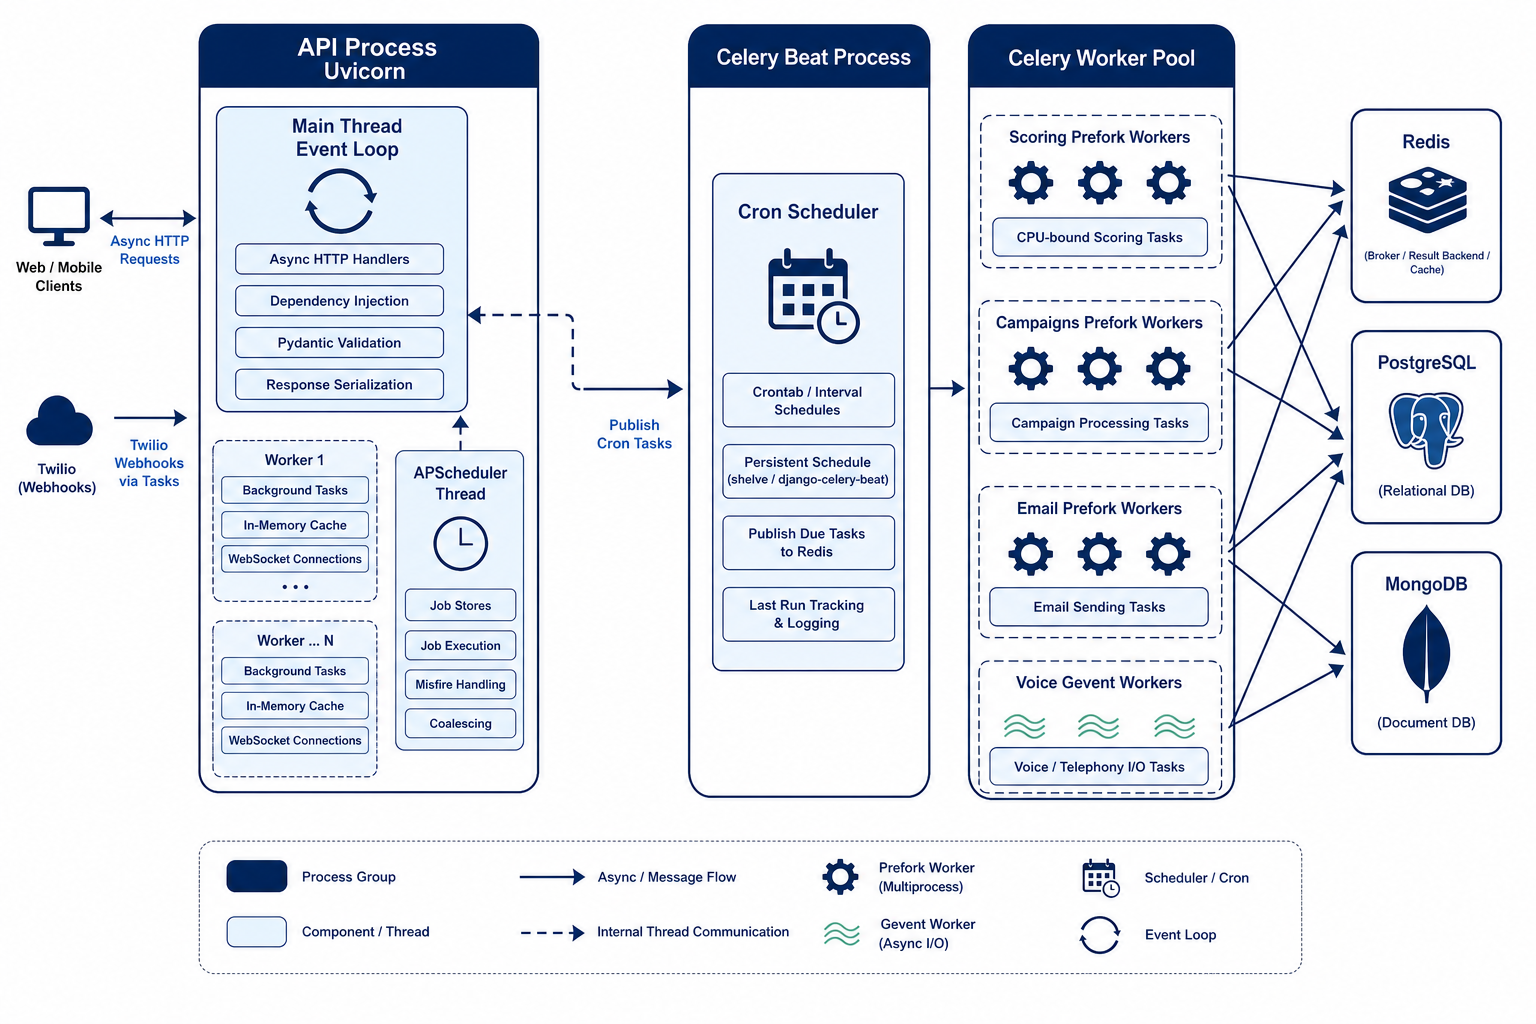
\includegraphics{images/rnu-async-runtime.png}%
    }
    \caption{Async runtime --- Uvicorn workers, Celery Beat, worker pools, and data store connections.}
    \label{fig:async}
\end{figure}
\end{landscape}

\FloatBarrier

% =============================================================================
\section{Cron \& Scheduled Jobs}

Each job uses an idempotency key, Redis distributed lock, dead-letter queue on failure, and \texttt{activity\_logs} entry in PostgreSQL.

\docfig{htbp}{0.38\textheight}{images/rnu-cron-scheduler.png}{Celery Beat cron catalog --- schedules, target queues, and lock semantics.}{fig:cron}

\Needspace{6\baselineskip}
\begin{tabularx}{\textwidth}{@{}L{3.6cm} L{3.4cm} p{2.4cm} Y@{}}
\toprule
\textbf{Job ID} & \textbf{Schedule (UTC)} & \textbf{Queue} & \textbf{Action} \\
\midrule
scoring\_daily & 0 0 * * * & scoring & Full portfolio scoring pipeline \\
scoring\_incremental & */6 * * * * & scoring & Accounts with activity in last 6h \\
lifecycle\_reclassify & after scoring jobs & scoring & Re-run fit-ratio bucket classifier with latest config \\
workflow\_step\_evaluator & */5 * * * * & workflows & Execute due \texttt{account\_workflow\_states} in send window \\
workflow\_enrollment\_sync & 0 1 * * * & workflows & Enroll accounts into quarter template on quarter change \\
campaign\_evaluator & */5 * * * * & campaigns & Evaluate due campaigns (IST windows) \\
email\_inbound\_poll & */2 * * * * & email & Poll provider if webhook unavailable \\
voice\_retry\_sweep & 0 */4 * * * & voice & Retry missed calls (+4h rule) \\
analytics\_rollup & 30 1 * * * & analytics & Refresh materialized views \\
integration\_sf\_sync & 0 2 * * * & integrations & Salesforce delta sync \\
mongo\_ttl\_cleanup & 0 3 * * 0 & maintenance & Verify TTL indexes \\
redis\_cache\_warm & 0 6 * * * & analytics & Pre-warm lifecycle dashboard cache \\
\bottomrule
\end{tabularx}

% =============================================================================
\section{API Surface}

REST prefix \texttt{/api/v1}. Webhooks use signature verification (no JWT).

\begin{longtable}{@{}p{3.8cm}p{3cm}p{5.5cm}@{}}
\toprule
\textbf{Prefix} & \textbf{Frontend Module} & \textbf{Key Endpoints} \\
\midrule
\endhead
/accounts & accounts.ts & GET/POST/PUT/DELETE, timeline, comments, ticket-stats \\
/lifecycle & lifecycle.ts & dashboard, accounts/\{id\}/agent, recommendation \\
/pipeline & Pipeline.tsx & GET grid (byQuarter, quarterTotals, stageCounts) \\
/analytics & analytics.ts & dashboard, portfolio, trends \\
/opportunities & opportunities.ts & CRUD upsell pipeline \\
/campaigns & pipeline UI & CRUD auto-campaigns, POST run-now \\
/email & email.ts & send, inbound webhook, trigger, preview, sentiment \\
/voice & voice.ts & calls, Twilio webhooks, trigger-calls \\
/whatsapp & whatsapp.ts & conversations, webhook, send-to-account \\
/ml & ml.ts & POST trigger (manual scoring) \\
/settings & settings.ts & app config, setup credentials, pause automation \\
/workflows & workflows.ts & templates/steps CRUD; topic, frequency, send windows \\
/voicebot & voicebot.ts & POST chat, WebSocket /ws, /audio/ws \\
/webhooks & --- & /twilio, /stripe, /salesforce, /email \\
\bottomrule
\end{longtable}

% =============================================================================
\section{Module Technical Flows}

\docfig{htbp}{0.30\textheight}{images/rnu-flow-campaign-tech.png}{Campaign technical flow --- PostgreSQL filter, Redis lock, Celery dispatch, channel router.}{fig:flow-campaign}

\docfig{htbp}{0.30\textheight}{images/rnu-flow-webhook-ingest.png}{Webhook ingest --- signature verify, Mongo archive, async Celery processing.}{fig:flow-webhook}

% =============================================================================
\section{Integration Layer}

\subsection{Twilio}
Voice outbound/inbound, SMS, WhatsApp. Webhooks: \texttt{/api/v1/voice/handle-call}, \texttt{handle-input}, \texttt{call-status}. Signature validation via \texttt{X-Twilio-Signature}.

\subsection{Email Provider}
Transactional send (Resend/SendGrid/SMTP). Inbound via webhook or 2-minute poll fallback. Raw body archived in Mongo; metadata in PostgreSQL.

\subsection{Salesforce}
Nightly delta sync (Celery \texttt{integration\_sf\_sync}). Bi-directional: accounts, contacts, opportunities. Sync log in \texttt{salesforce\_sync\_log}.

\subsection{Stripe}
Webhook for payment completion $\rightarrow$ update account status, create transaction row, trigger renewal event.

% =============================================================================
\section{Security \& Governance}

\begin{itemize}[leftmargin=1.5em, itemsep=0.3em]
    \item \textbf{Authentication:} JWT (HS256/RS256), 30-minute access token, refresh token in HTTP-only cookie
    \item \textbf{Authorization:} RBAC roles --- admin, csm, viewer; enforced via FastAPI dependencies
    \item \textbf{Tenancy:} Every query scoped by \texttt{tenant\_id} from JWT claims
    \item \textbf{Secrets:} Integration credentials encrypted at rest (\texttt{pgcrypto}); never plaintext in app\_settings
    \item \textbf{Audit:} activity\_logs for scoring runs, campaign executions, status changes, manual triggers
    \item \textbf{Human gates:} Protect-stage outreach and churn marking require CSM approval (NBA graph gate)
    \item \textbf{Rate limits:} Redis token bucket per tenant for LLM and Twilio
\end{itemize}

% =============================================================================
\section{Deployment Topology}

\docfig{htbp}{0.45\textheight}{images/rnu-deployment-topology.png}{Production deployment --- load balancer, API/WebSocket nodes, data stores, Celery workers.}{fig:deploy}

\textbf{Observability:}
\begin{itemize}[leftmargin=1.5em, itemsep=0.2em]
    \item Structured JSON logs (request\_id, tenant\_id, trace\_id)
    \item OpenTelemetry spans on LangGraph nodes and Celery tasks
    \item Prometheus metrics: queue depth, scoring duration, webhook latency
    \item Health endpoints: \texttt{/health}, \texttt{/ready} (PostgreSQL + Redis checks)
\end{itemize}

% =============================================================================
\section{Implementation Phases}

\begin{longtable}{@{}p{2.5cm}p{5cm}p{5cm}@{}}
\toprule
\textbf{Phase} & \textbf{Scope} & \textbf{Exit Criteria} \\
\midrule
\endhead
0 --- Foundation & PostgreSQL schema (Alembic), FastAPI skeleton, JWT, Redis & Accounts CRUD on real PostgreSQL \\
1 --- Intelligence & Formula scoring + LiteLLM sentiment; DB-driven scoring\_formulas config; daily cron & Dashboard shows live formula-based scores; Settings edits thresholds \\
1b --- ML swap (future) & Per-node ML via SCORING\_MODE=ml; joblib models & Same API; history logs scoring\_mode \\
2 --- Lifecycle \& Grid & Fit-ratio bucket engine, pipeline grid API, 5-bucket filter, Redis cache & /lifecycle/dashboard and /pipeline/grid match frontend \\
3 --- Dynamic Workflows & Workflow template CRUD, account\_workflow\_states, Resend + Twilio executor & End-to-end Q1 workflow run (email + voice) \\
4 --- Outreach \& Integrations & Campaign service, Salesforce/Stripe, workflow analytics & Campaigns + executive analytics live \\
\bottomrule
\end{longtable}

% =============================================================================
\section{Appendix: Diagram Maintenance}

Mermaid source specifications: \texttt{diagrams/README.md}.\\
LLM image regeneration prompts: \texttt{diagrams/IMAGE\_PROMPTS.md}.\\
PostgreSQL reference DDL: \texttt{schemas/postgres.ddl}.\\
Phase~1 scoring formulas: \texttt{schemas/scoring\_formulas.md}.\\
Scoring config defaults: \texttt{schemas/scoring\_config.example.json}.

\vspace{1.5em}
\begin{center}
    {\color{brandblue}\rule{0.6\textwidth}{1.5pt}}\\[0.5em]
    \textit{PostgreSQL \textperiodcentered\ Redis \textperiodcentered\ MongoDB \textperiodcentered\ LangGraph}\\[0.3em]
    \textbf{\color{brandblue}Built for Production Revenue Operations}
\end{center}

\end{document}
